\chapter{Thesis Plan}
\label{ch:project_plan}
In the following section, the thesis plan of the proposed master's thesis is discussed.
The thesis plan consists of a work plan and risk assessment.
The work plan defines the thesis objectives, milestones, tasks, and deliverables and is presented in \autoref{sec:work_plan}.
The time schedule represents the mapping of the proposed work plan to Calendar Weeks (CW) and is visualized in \autoref{fig:timeplan}.
The risk assessment evaluates technical and non-technical risks for the proposed thesis plan and is discussed in \autoref{sec:risk_assessment}.

\section{Work Plan}
\label{sec:work_plan}
%\todo{Workplan, Incremental Parts ("inkremente"), Dependencies, Deliverable-Duration-Limitation, time schedule (milestones, temporal dependencies)}
The work plan structures the proposed thesis into six milestones.
Each milestone represents a major phase of the proposed master's thesis.
The milestones serve as intermediate thesis goals which enable monitoring and reporting of thesis progress.
Each milestone is defined by its duration in CWs, deliverables, and tasks.
Each milestone consists of at least one task.
A task of a milestone is referred to as increment.
The duration of a milestone depends on the duration of its increments and increment interdependencies.
Multiple increments mapped to the same calendar weeks may be performed in parallel, as there are either no interdependencies or existing dependencies can be resolved beforehand.
The projected timescales for the completion of milestones and increments are calculated based on empirical values.
The milestones of the proposed master's thesis are defined as follows:
\begin{description}
    \item[Milestone I:] Preliminary Work
    \begin{description}[style=multiline, leftmargin=\widthof{\textbf{Deliverables:}}]
        \item[Duration:] 14 Weeks (15. April 2024 (CW 16) -- 22. July 2024 (CW 30))
        \item[Deliverables:] Master's thesis proposal
    \end{description}
    \item[Milestone II:] Realization
    \begin{description}[style=multiline, leftmargin=\widthof{\textbf{Deliverables:}}]
        \item[Duration:] 11 Weeks (22. July 2024 (CW 30) -- 07. October 2024 (CW 41))
        \item[Deliverables:]
        \begin{enumerate}[label=\alph*), leftmargin=\widthof{a)}+\labelsep]
            \item Software Design, Implementation, Tests (Unit, Integration, and System), \& Test Coverage Report of CASC-SAS
            \item Hardware Deployment Scripts of CASC-SAS
            \item Thesis Chapter: Realization
        \end{enumerate}
        \item[Increments:]
        \begin{enumerate}[label=\arabic*), leftmargin=\widthof{a)}+\labelsep]
            \item Design, Implementation, Tests, \& Deployment of SABAAC (7 Weeks)
            \item Design, Implementation, Tests, \& Deployment of CASA (7 Weeks)
            \item Architecture \& Code Review (Optional, Single Meeting)
            \item Writing of Documentation (2 Weeks)
        \end{enumerate}
    \end{description}
    \item[Milestone III:] Evaluation
    \begin{description}[style=multiline, leftmargin=\widthof{\textbf{Deliverables:}}]
        \item[Duration:] 7 Weeks (07. October 2024 (CW 41) -- 25. November 2024 (CW 48))
        \item[Deliverables:]
        \begin{enumerate}[label=\alph*), leftmargin=\widthof{a)}+\labelsep]
            \item Evaluation Results of CASC-SAS
            \item Thesis Chapter: Evaluation
        \end{enumerate}
        \item[Increments:]
        \begin{enumerate}[label=\arabic*), leftmargin=\widthof{a)}+\labelsep]
            \item Security Evaluation (3 Weeks)
            \item Performance Evaluation (3 Weeks)
            \item Compatibility Evaluation (1 Weeks)
            \item Writing of Documentation (2 Weeks)
        \end{enumerate}
    \end{description}
    \item[Milestone IV:] Conclusion
    \begin{description}[style=multiline, leftmargin=\widthof{\textbf{Deliverables:}}]
        \item[Duration:] 2 Weeks (25. November 2024 (CW 48) -- 09. December 2024 (CW 50))
        \item[Deliverables:]
        \begin{enumerate}[label=\alph*), leftmargin=\widthof{a)}+\labelsep]
            \item Thesis Chapter: Conclusion
            \item Thesis Chapter: Limitations
            \item Thesis Chapter: Future Work
            \item Thesis Chapter: Abstract
        \end{enumerate}
        \item[Increment:] Writing of Documentation: Conduct a review of results and derive a conclusion, limitations, and future work with regard to the research questions (2 Weeks)
    \end{description}
    \item[Milestone V:] Review
    \begin{description}[style=multiline, leftmargin=\widthof{\textbf{Deliverables:}}]
        \item[Duration:] 5 Weeks (09. December 2024 (CW 50) -- 13. January 2025 (CW 03))
        \item[Deliverables:] Reviewed \& Proofread Master's Thesis
        \item[Increments:]
        \begin{enumerate}[label=\arabic*), leftmargin=\widthof{a)}+\labelsep]
            \item Internal Review: Proofreading \& Correction by the Authors (2 Weeks)
            \item External Review: Proofreading \& Correction by External Readers (4 Weeks)
        \end{enumerate}
    \end{description}
    \item[Milestone VI:] Finalization
    \begin{description}[style=multiline, leftmargin=\widthof{\textbf{Deliverables:}}]
        \item[Duration:] 6 Weeks (09. December 2024 (CW 50) -- 20. January 2025 (CW 04))
        \item[Deliverables:]
        \begin{enumerate}[label=\alph*), leftmargin=\widthof{a)}+\labelsep]
            \item Printed \& Bound Master's Thesis
            \item Master's Thesis Presentation Slides
        \end{enumerate}
        \item[Increments:]
        \begin{enumerate}[label=\arabic*), leftmargin=\widthof{a)}+\labelsep]
            \item Thesis Presentation Preparation (5 Weeks)
            \item Printing \& Binding of Thesis (1 Week)
        \end{enumerate}
    \end{description}
\end{description}
\begin{figure}
    \centering
    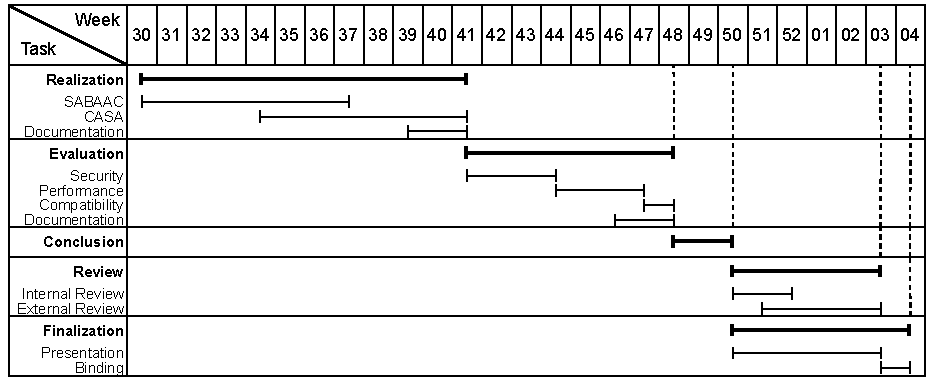
\includegraphics[width=1.0\linewidth]{figures/timeplan.drawio.pdf}
    \caption{Time schedule of the proposed master's thesis.}
    \label{fig:timeplan}
\end{figure}

\section{Risk Assessment}
\label{sec:risk_assessment}
The risk assessment identifies potential risks and assesses their impact on the proposed thesis plan.
Additionally, it presents mitigation strategies for the identified risks.
By considering the occurrence of undesirable events, the risk assessment enables the meeting of deadlines.
The identified and assessed risks are classified as either technical or non-technical risks.
The technical risks are discussed in detail in \autoref{sec:risk_assessment_technical}.
The non-technical risks consist of organizational and project management risks and are discussed in detail in \autoref{sec:risk_assessment_project_management}.

\subsection{Technical Risks}
\label{sec:risk_assessment_technical}
The following technical risks represent deficiencies in the design and implementation of the approach, which could result in non-compliance with stated requirements.
To ensure the compliance with stated requirements, it is recommended that software testing and system evaluation are conducted in an automated manner.
\begin{description}
    \item[Software Design Flaws] Software design flaws have an impact on the performance, availability, security, and safety of the approach.
    To mitigate the risk of software design flaws and therefore avoid re-implementation, architecture reviews are conducted after the design of the CASC-SAS software.
    Furthermore, automated acceptance tests check the compliance of already implemented software with stated system requirements to identify software design flaws.
    \item[Software Implementation Flaws] Software implementation flaws have an impact on the performance, availability, security, and safety of the approach.
    Implementation flaws such as bugs are avoided by using automated software testing.
    The automated software testing consists of unit, integration, system, and acceptance tests.
    The unit, integration, and system tests assure the correct and failure-free operation of the software under valid and invalid system conditions.
    The acceptance tests check the compliance with stated system requirements.
    The employed software testing methods have to provide high source code coverage.
    Besides automated software testing, code reviews after the implementation of the CASC-SAS software can increase the source code quality and mitigate the risk of implementation flaws.
    \item[Transient Hardware Faults] Transient faults of system hardware have an impact on the performance and availability of the approach.
    Transient faults have to be taken into account during the design and implementation of the system.
    This can be achieved by employing failure-avoidance strategies such as redundancy and automated system monitoring.
    \item[Persistent Hardware Faults] Persistent faults of system hardware have an impact on the performance and availability of the approach.
    Persistent faults have to identified via automated system monitoring and resolved by replacing corresponding hardware components.
    \item[Unsuitable Hardware] Unsuitable hardware has an impact on the performance and economic aspects of the approach.
    As a consequence, unsuitable hardware has to be replaced by suitable hardware to satisfy the system requirements.
    To make the approach performant and economically feasible, the system has to use components that provide neither too much nor too less performance for their designated tasks.
\end{description}

\subsection{Organizational \& Project Management Risks}
\label{sec:risk_assessment_project_management}
The following risks represent deficiencies in the project organization and management.
To mitigate the following risks, a preliminary milestone was created with the objective of reducing the number and complexity of tasks to be completed within the limited thesis period.
\begin{description}
    \item[Inaccurate Estimation of Milestone \& Increment Duration] The projected durations of milestones and increments are calculated based on empirical values.
    However, this calculation approach may result in inaccurate estimations, which could lead to a deviation from the proposed time schedule.
    To mitigate the risk of inaccurate estimations, an additional buffer time is included in each duration associated with an increment or milestone.
    \item[Illness-Related Delay] Illness may result in a deviation from the proposed time schedule.
    Small deviations, in the order of weeks, can be compensated by the additional buffer times.
    Large deviations, in the order of months, require either an extension of the limited thesis period or a prioritization of increments.
    The possibility of extending the thesis period by up to three months is governed by the examination regulations.
\end{description}
